%% UzK - A BEAMER THEME FOR THE UNIVERSITY OF COLOGNE
%% http://solstice.github.com/uzk-theme/

\documentclass{beamer}
\usepackage[ngerman]{babel}
%\usepackage[latin1]{inputenc}
\usepackage[T1]{fontenc}
\usepackage{xltxtra} 
\defaultfontfeatures{Mapping=tex-text}


%% Falls Anzeige der \sections, \subsections etc. gewuenscht, kann zB.
%% das infolines theme geladen werden. Wichtig ist jedoch, dass andere
%% Themes _vor_ dem UzK-Theme geladen werden.
%\useoutertheme{infolines}

%% Falls keine der Optionen zur Bestimmung der Fusszeile uebergeben werden    %%
%% werden alle Fakultaetsfarben verwendet. ---------------------------------- %%
\usetheme[%
%wiso,        %% Wiso-Fakultaet
%jura,        %% Rechtswissenschaftliche Fakultaet
medizin,     %% Medizinische Fakultaet
%philo,       %% Philosophische Fakultaet
%matnat,      %% Mathematisch-Naturwissenschaftliche Fakultaet
%human,       %% Humanwissenschaftliche Fakultaet
%verw,        %% Universitaetsverwaltung
%nav,         %% Schaltet die Navigationssymbole ein
%latexfonts,  %% Verwendet die latex-beamer-Standardschrift
%colorful,    %% Farbige Balken im infolines-Theme
%squares,     %% Aufzaehlungspunkte rechteckig
]{UzK}

\title{VeriSO -- Verifikation von Interlis-Daten}

\author[Stefan Ziegler]%
{Stefan Ziegler}%
  

\institute[Amt für Geoinformation]{%
Amt für Geoinformation \\
Rötistrasse 4\\
4500 Solothurn}

\date[07.11.13]{07. November 2013}
\begin{document}

\begin{frame}
  \titlepage
\end{frame}

\begin{frame}
  \frametitle{Inhalt}
  \begin{itemize}
  \item Datenverwaltung
  \item Interlis-Import
  \item QGIS-GUI
  \item Checks
  \item Checkliste
  \end{itemize}
\end{frame}

\begin{frame}
  \frametitle{Einleitung}
  \begin{itemize}
  \item Ausgangslage: 
  \begin{itemize}
   \item Viele \textit{einzelne} Operate in \textit{einheitlichem} Datenmodell.
   \item Z.B. Amtliche Vermessung, Nutzungsplanung, Naturgefahren etc. 
   \item Daten müssen verifiziert werden.
  \end{itemize}

  \item Ziel: 
  \begin{itemize}
   \item Generisch, d.\,h. nicht nur für amtliche Vermessung sondern für alle Daten, die mit Interlis erfasst sind.
   \item Keine technische Anpassungen für neues Datenmodell.
   \item Fokus der Anpassung auf Checks.
  \end{itemize}  
    \end{itemize}
\end{frame}

\begin{frame}
  \frametitle{Datenverwaltung}
  \begin{itemize}
  \item Pro zu verifizierendes Datenmodell ein (1) Datenbankschema, d.\,h. alle Gemeinden und sämtliche Lieferungen in einem Schema.
  \item Z.\,B. für Verifikation der DM.01-Aufarbeitung und Gebäudeadressen: \texttt{av\_dm01avso24}
  \item Identifizierbarkeit? Eindeutigkeit?
  \item Jedem Objekt wird \texttt{gem\_bfs}, \texttt{lieferdatum} und \texttt{los} beim Import hinzugefügt.
  \end{itemize}
\end{frame}

\begin{frame}
  \frametitle{Datenverwaltung}
  \begin{figure}
    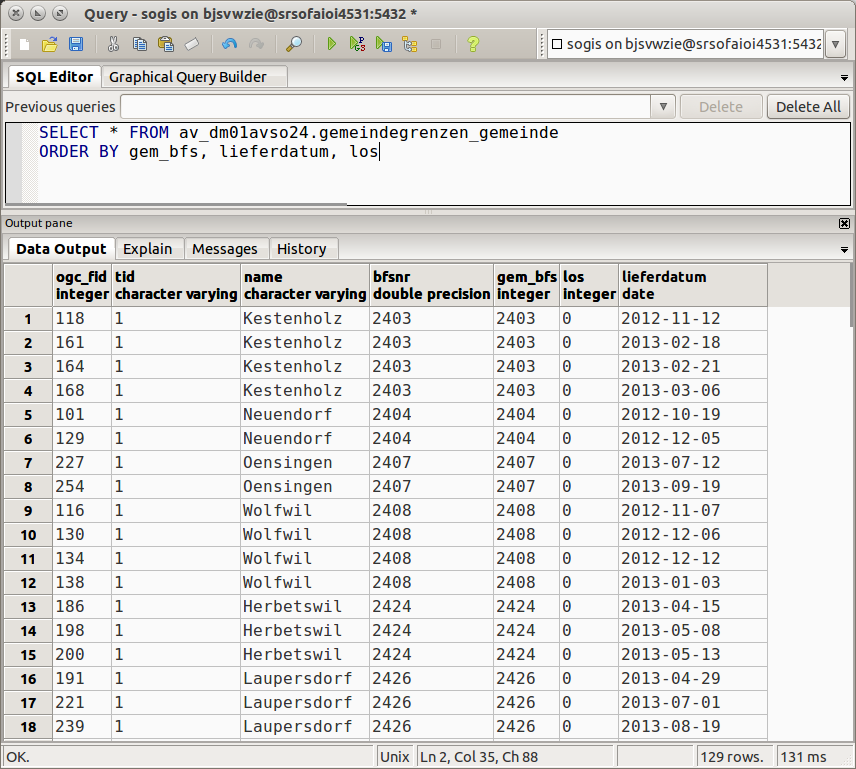
\includegraphics[scale=0.25]{bilder/veriso_liste_gemeinden_2.png}
  \end{figure}
\end{frame}

\begin{frame}
  \frametitle{Interlis-Import}
  \begin{itemize}
  \item Java: \textbf{iox-ili} für Interlis, \textbf{GeoTools} für alles andere (z.\,B. Import in Datenbank).
  \item Segmentierung und Polygonierung während des Importprozesses.
  \item 1:1-Transfer, (fast) kein Datenumbau:
  \begin{itemize}
   \item Attribute hinzufügen: \texttt{gem\_bfs}, \texttt{lieferdatum} und \texttt{los}
   \item Aufzähltypen werden zusätzlich ausgeschrieben:
   \begin{itemize}
    \item \texttt{art} $\rightarrow$ \texttt{art\_txt}
    \item \texttt{1} $\rightarrow$ \texttt{befestigt.Strasse\_Weg}
   \end{itemize}
  \end{itemize}
 \end{itemize}
\end{frame}


\begin{frame}
  \frametitle{QGIS-GUI}
  \begin{figure}
    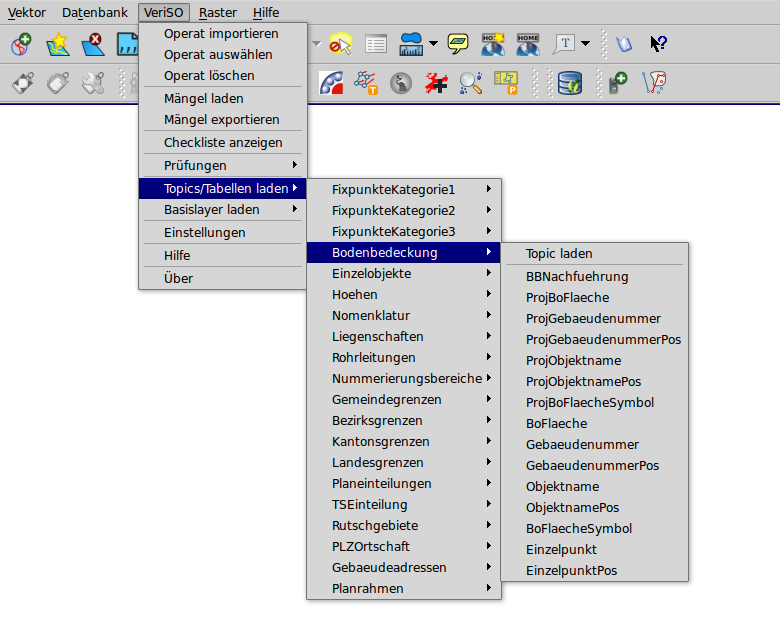
\includegraphics[scale=0.35]{bilder/veriso_topic_loader_3.png}
  \end{figure}
\end{frame}

\begin{frame}
  \frametitle{QGIS-GUI}
  \begin{figure}
    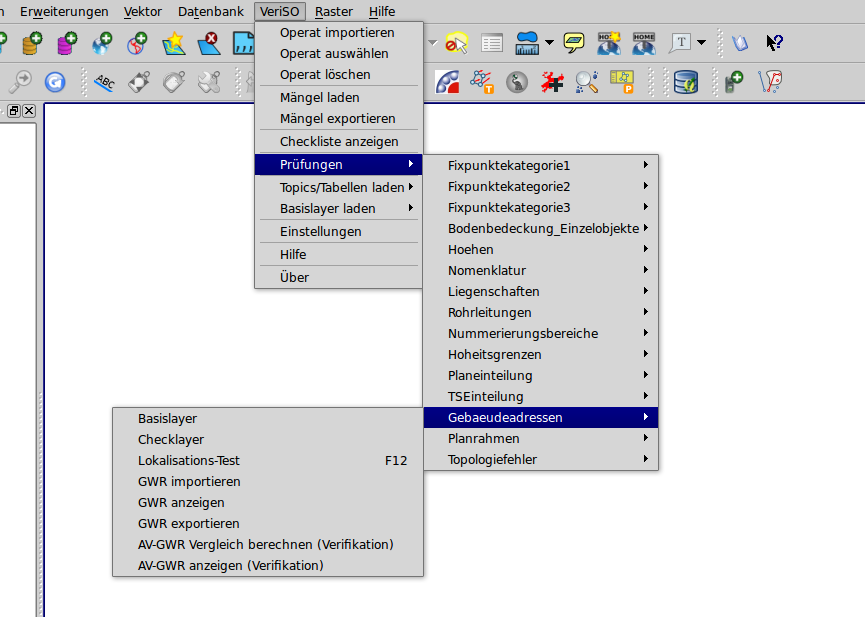
\includegraphics[scale=0.35]{bilder/veriso_checks_3.png}
  \end{figure}
\end{frame}

\begin{frame}[fragile]
  \frametitle{QGIS-GUI: ILI $\rightarrow$ XML}
  \begin{tiny}
  \begin{verbatim}
<?xml version="1.0" encoding="ISO-8859-1"?>
<topics>
  <topic id="FixpunkteKategorie1" title="FixpunkteKategorie1" group="FixpunkteKategorie1">
    <table>
      <group>FixpunkteKategorie1</group>
      <title>LFP1Nachfuehrung</title>
      <schema>av_dm01avso24</schema>
      <table>fixpunktekategorie1_lfp1nachfuehrung</table>
      <geom>perimeter</geom>
      <style></style>
    </table>
    <table>
      <group>FixpunkteKategorie1</group>
      <title>LFP1</title>
      <schema>av_dm01avso24</schema>
      <table>fixpunktekategorie1_lfp1</table>
      <geom>geometrie</geom>
      <style></style>
    </table>
    ....
  <topic id="Bodenbedeckung" title="Bodenbedeckung" group="Bodenbedeckung">   
    <table>
      <group>Bodenbedeckung</group>
      <title>BoFlaeche</title>
      <schema>dm01avso24</schema>
      <table>bodenbedeckung_boflaeche</table>
      <geom>geometrie</geom>
      <style></style>
    </table>
    ....
 </topic>
</topics>    
  \end{verbatim}
  \end{tiny}
\end{frame}


\begin{frame}[fragile]
  \frametitle{QGIS-GUI: XML für Checks}
  \begin{tiny}
  \begin{verbatim}
<?xml version="1.0" encoding="ISO-8859-1"?>
<checks>
  <check id="fixpunktekategorie1" title="Übersicht" group="Fixpunktekategorie1" 
         topic="Fixpunktekategorie1" type="complex">
    <file>complexchecks.fp1</file>
  </check>
  ...  
  <check id="gebaeudeadressen_basis" title="Basislayer" group="Gebaeudeadressen - Basislayer" 
         topic="Gebaeudeadressen" type="complex">
    <file>complexchecks.gebaeudeadressen_basislayer</file>
  </check>   
  <check id="gebaeudeadressen_check" title="Checklayer" group="Gebaeudeadressen - Checklayer" 
         topic="Gebaeudeadressen" type="complex">
    <file>complexchecks.gebaeudeadressen_checklayer</file>
  </check>    
  <check id="gebaeudeadressen_lokalisations" title="Lokalisations-Test" 
         group="Gebaeudeadressen - Lokalisations-Test" topic="Gebaeudeadressen" type="complex">
    <file>complexchecks.gebaeudeadressen_lokalisation</file>
    <shortcut>F12</shortcut>
  </check>           
  ...
</checks>   
  \end{verbatim}
  \end{tiny}
\end{frame}

\begin{frame}[fragile]
  \frametitle{Checks}
  \begin{itemize}
  \item «Alles ist möglich!»
  \item «einfach»:
  \begin{itemize}
   \item Vordefinierte PostGIS-Views oder Tabellen (falls View zu langsam).
   \item Tabellen werden während des Importes abgefüllt.
   \item Queries sind in spezieller Tabelle gespeichert. 
  \end{itemize}
  \item «komplex»:
  \begin{itemize}
   \item beliebig kompliziert
   \item Alles was die Python- und PyQGIS-API hergibt, z.\,B.:
   \begin{itemize}
    \item Excel-Export
    \item PDF erzeugen
    \item Daten mit WFS requesten und vergleich.
    \item \ldots
   \end{itemize}

  \end{itemize}
  
  \item Alles in \textit{mindestens} einer Python-Datei verpackt.
 \end{itemize}
\end{frame}

\begin{frame}
  \frametitle{Checks}
  \begin{figure}
    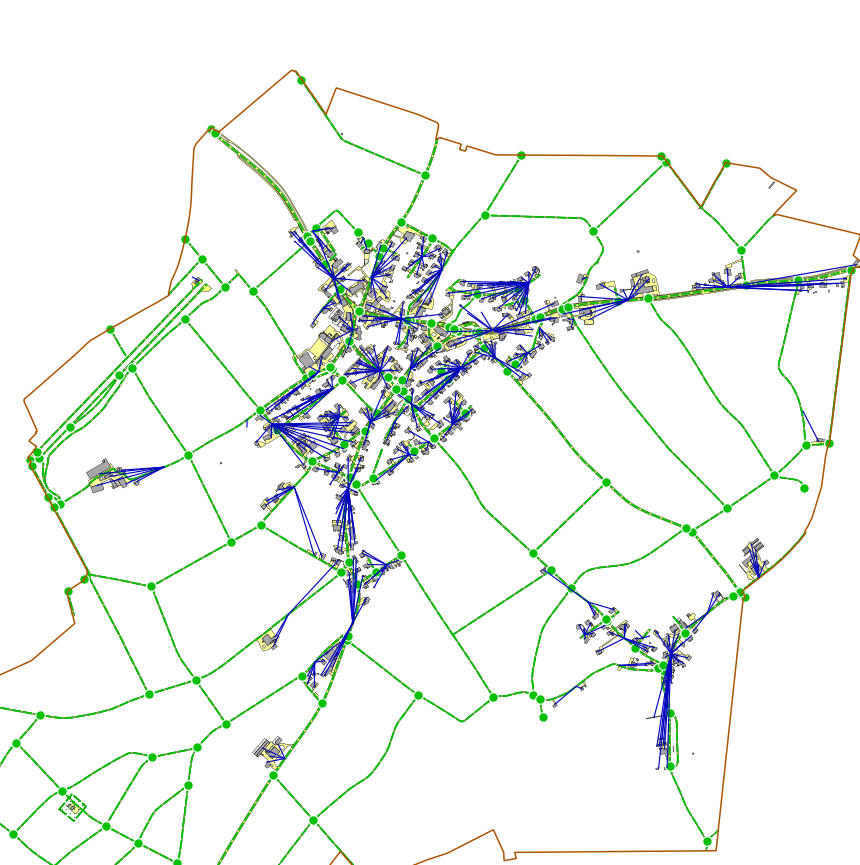
\includegraphics[scale=0.3]{bilder/veriso_spinnennetz_1.png}
  \end{figure}
\end{frame}

\begin{frame}
  \frametitle{Checks}
  \begin{figure}
    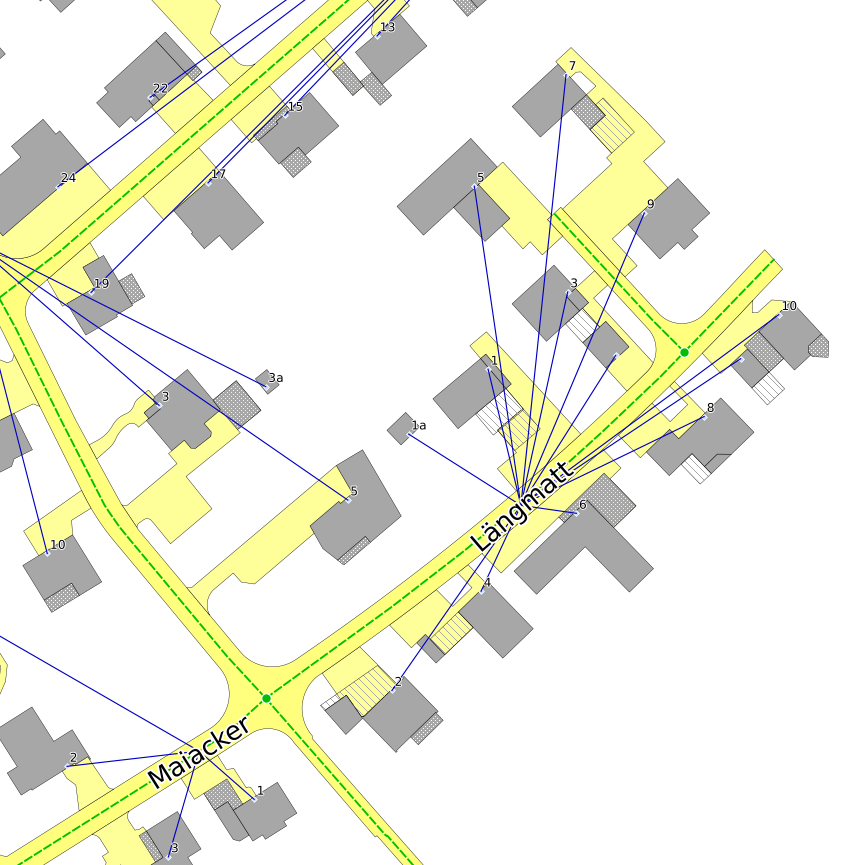
\includegraphics[scale=0.3]{bilder/veriso_spinnennetz_2.png}
  \end{figure}
\end{frame}

\begin{frame}
  \frametitle{Checks}
  \begin{figure}
    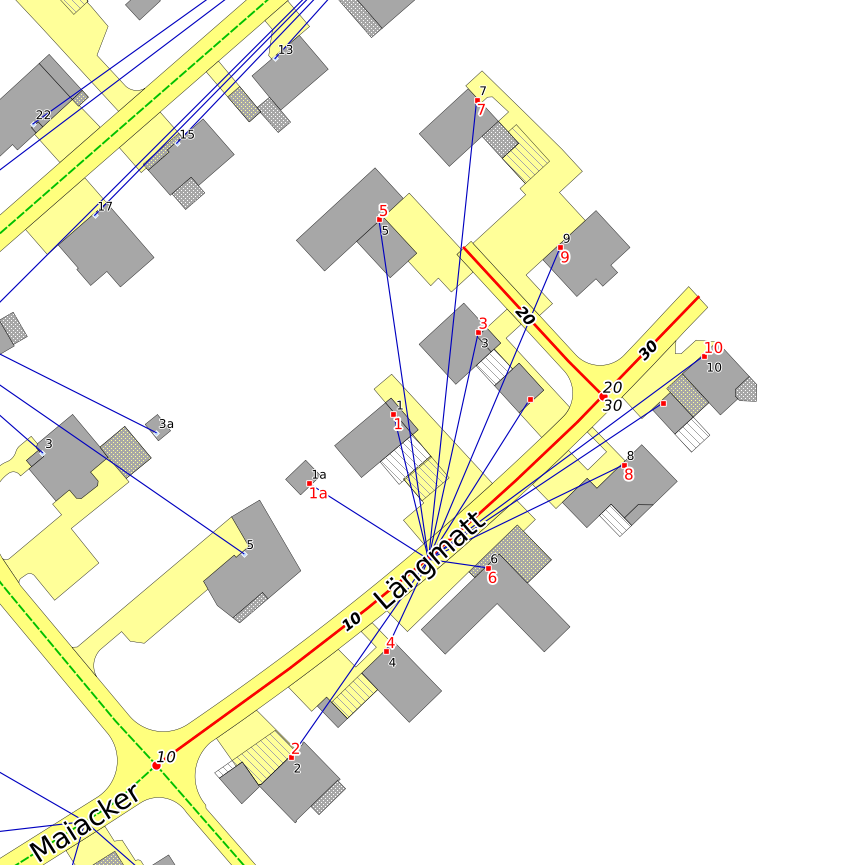
\includegraphics[scale=0.3]{bilder/veriso_f12.png}
  \end{figure}
\end{frame}

\begin{frame}
  \frametitle{Checks}
  \begin{figure}
    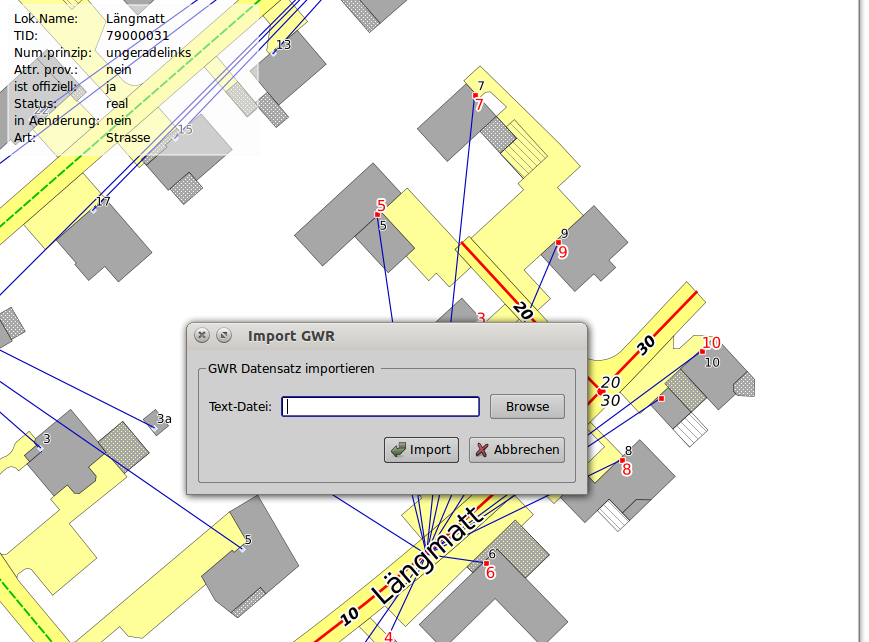
\includegraphics[scale=0.3]{bilder/veriso_gwr_import.png}
  \end{figure}
\end{frame}

\begin{frame}[fragile]
  \frametitle{Checks: Umsetzung GUI}
  \begin{tiny}
  \begin{verbatim}
<?xml version="1.0" encoding="ISO-8859-1"?>
<checks>
  <check id="fixpunktekategorie1" title="Übersicht" group="Fixpunktekategorie1" 
         topic="Fixpunktekategorie1" type="complex">
    <file>complexchecks.fp1</file>
  </check>
  ...  
  <check id="gebaeudeadressen_basis" title="Basislayer" group="Gebaeudeadressen - Basislayer" 
         topic="Gebaeudeadressen" type="complex">
    <file>complexchecks.gebaeudeadressen_basislayer</file>
  </check>   
  <check id="gebaeudeadressen_check" title="Checklayer" group="Gebaeudeadressen - Checklayer" 
         topic="Gebaeudeadressen" type="complex">
    <file>complexchecks.gebaeudeadressen_checklayer</file>
  </check>    
  <check id="gebaeudeadressen_lokalisations" title="Lokalisations-Test" 
         group="Gebaeudeadressen - Lokalisations-Test" topic="Gebaeudeadressen" type="complex">
    <file>complexchecks.gebaeudeadressen_lokalisation</file>
    <shortcut>F12</shortcut>
  </check>           
  ...
</checks>   
  \end{verbatim}
  \end{tiny}
\end{frame}

\begin{frame}
  \frametitle{Checks: Umsetzung GUI}
  \begin{figure}
    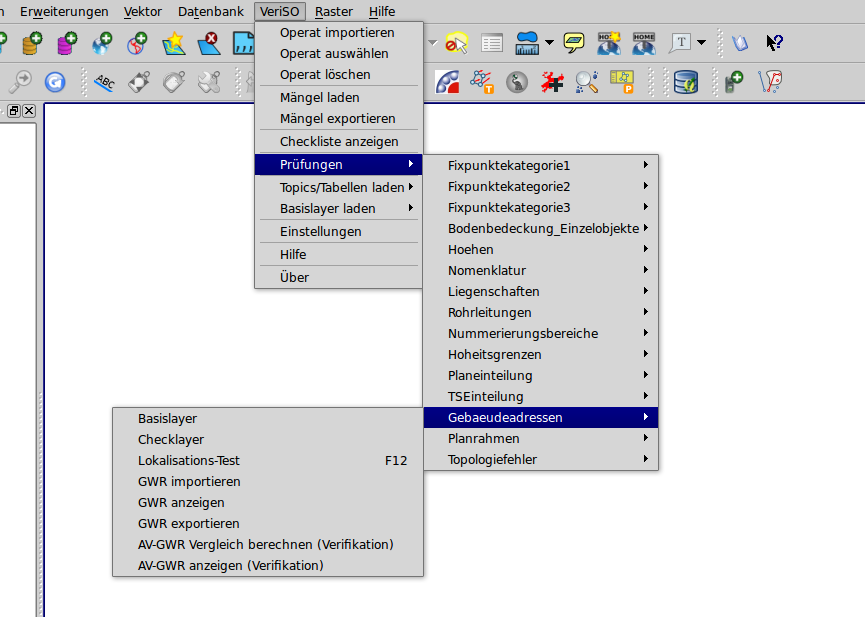
\includegraphics[scale=0.35]{bilder/veriso_checks_3.png}
  \end{figure}
\end{frame}




\begin{frame}[fragile]
  \frametitle{Checkliste}
  \begin{itemize}
  \item Möglichst einfach.
  \item Keine zusätzliche Software.
  \item HTML-Formulare
  \item Persistentes Speichern von Daten mittels \textit{Web Storage}.
  \item Achtung: Daten «nur» im Browser gespeichert!
  \item Für jedes Operat wird HTML-Datei von Template kopiert.
  \end{itemize}
\end{frame}





\end{document}
